\documentclass[number]{assignment}
\usepackage{titlepage}
\usepackage{ncolor}
\usepackage{math}
\usepackage{enumitem}
\usepackage{multicol}
\usepackage{float}
\usepackage{pdflscape}

\setprimary{orange}

\name{Daniel}{Fitzmaurice}
\studentnumber{43961229}
\coursecode{deco2800}

\linespread{1.1}
\setlength{\columnseprule}{0.4pt}

\begin{document}
\begin{landscape}
\headfoot
\begin{multicols}{3}

\heading{Team}
Complementary Skills; Mutual Accountability; Common Commitment; Shared Goal; Collective Work Products; More than the sum of its parts\\
\subheading{Meetings}
Hogging -- talking too much; Flogging -- beating an issue to death; Frogging -- jumping from topic to topic; Bogging -- getting stuck on an issue; Ignoring the Elephant in the Corner\\
\heading{Software Architecture}
\subheading{Quality}
Cohesion -- Degree to which elements of a module fit together\\
Coupling -- Degree of interdependence between modules\\
\begin{multicols}{2}
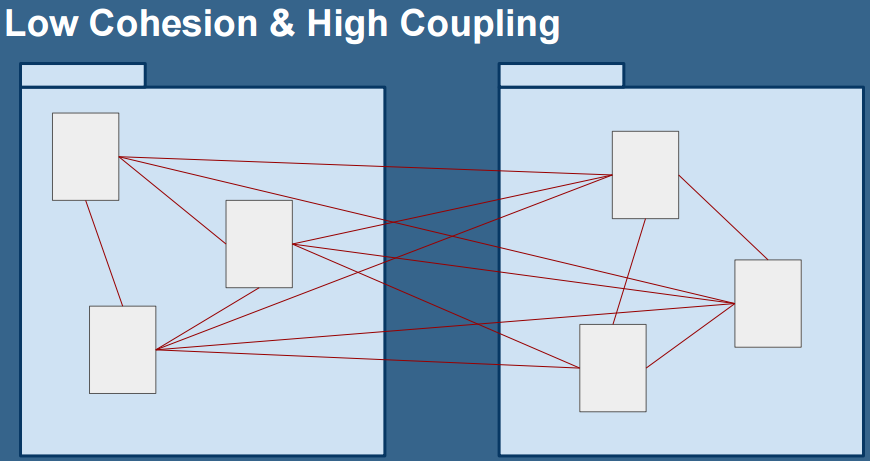
\includegraphics[width=\linewidth]{LowCHighC.png}
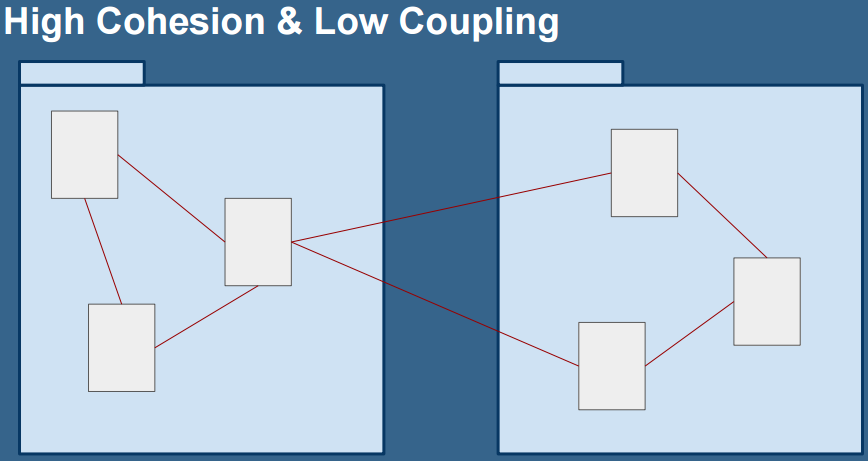
\includegraphics[width=\linewidth]{HighCLowC.png}
\end{multicols}
\heading{Continuous Integration}
Merge Frequently; Don't push broken code; Don't push untested code; Don't push when the build is broken; If the build is broken, fix it\\
\heading{Test-Driven Development}
A software development methodology based on: Short development iterations, Satisfying pre-prepared test cases. An independent offshoot of Agile methodologies. Based on using automated unit testing to drive software development.
\begin{multicols}{2}
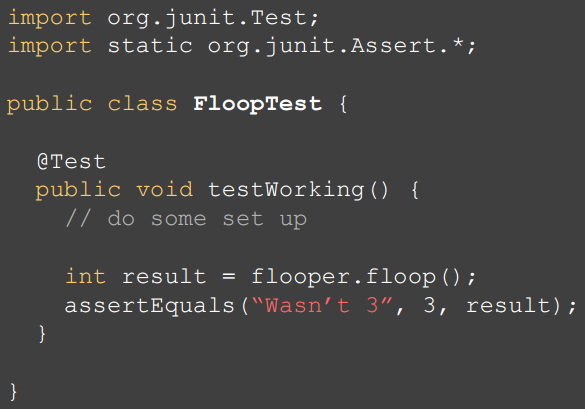
\includegraphics[width=\linewidth]{test1.png}
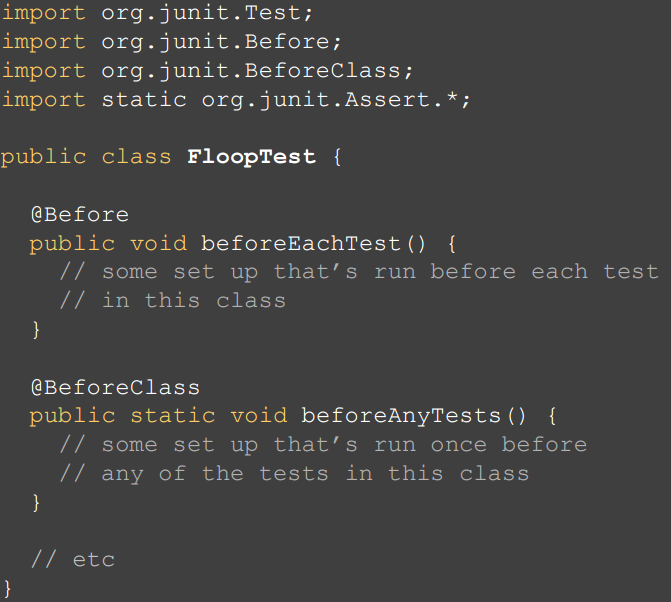
\includegraphics[width=\linewidth]{test2.png}
\end{multicols}
\subheading{Test-Driven Dev: Red, Green, Refactor}
\begin{multicols}{2}
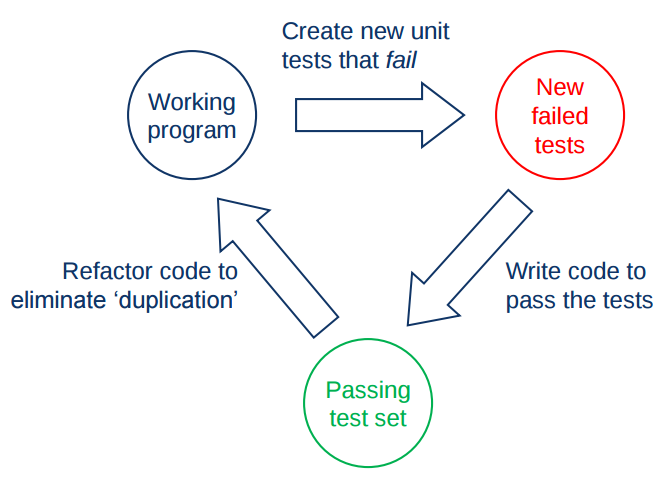
\includegraphics[width=\linewidth]{Cycle.png}
Applying Test-Driven Development relies on the existence of an automated unit testing environment. You are obliged to maintain a suite of test cases. Code must not be released until is has associated tests. The test are written \textbf{before} the code.
\end{multicols}
\subheading{Refactoring}
Code that needs refactoring has: Duplication, Unclear intent, Tight coupling, Pure data classes, Over-sized or under-sized classes, Complex or long methods, Switch statements instead of polymorphism.
\subheading{Designing Unit Tests}
Test one thing only (Use few assertions per test). Work in isolation (Without relying on other tests). Test boundary conditions early. Avoid testing against ``real'' resources, i.e. GUIs or databases, to support testing determinism (Use mock objects and services - with fixed data)
\subsubheading{How Many Tests?}
Test or both black-box and glass-box. As the programmer add glass-box tests for: Conditionals, Loops, Operations, Polymorphism.
\subheading{Mocking}
\textbf{\firstletter{D}ummies} - test objects which are never used but exist only to satisfy syntactic requirements\\
\textbf{\firstletter{S}tubs} - test objects whose methods return fixed values, and support the specific test cases only\\
\textbf{\firstletter{F}akes} - test objects whose methods work but have only limited functionality\\
\textbf{\firstletter{M}ocks} - test object which know how they're meant to be used, e.g. the sequence in which their methods should be called (allowing behavioural verification instead of just state verification)
\heading{Pair Programming}
Constant review from two people ensures fewer defects. Works well for mentoring: inexperienced staff, new team members, learning new techniques or tools.\\
\textbf{\firstletter{D}river} - person at the keyboard\\
\textbf{\firstletter{N}avigator} - focusing on design\\
Both need to be actively engaged - keep a running commentary\\
Switch roles frequently - every few minutes
\subheading{Ping-Pong Programming}
Driver writes a failing unit test. Driver \& Navigator switch roles. New driver implements code to pass test - then write a new failing unit test. Switch roles again
\heading{Class Model}
\subheading{Class Icon}
\begin{tabular}{|l|}
\hline
Employee \texttt{(Class Name)}\\\hline
-employeeNumber:String \texttt{(Attribute)}\\
-\underline{nextEmployeeNumber:String} \texttt{(Static Attribute)}\\
-qualification:Qualification[]\\\hline
+addQualification(qual:Qualification) \texttt{(Operation)}\\
+getDepartment():Department\\
+changeDepartment(dept:Department)\\\hline
\end{tabular}

\heading{System}
Jenkins -- Builds the changes to the repo; SonarQube -- checks for codesmells and code errors; Gradle -- For testing and running on local machine\\

\end{multicols}
\end{landscape}
\end{document}